\documentclass{article}

\usepackage{ctex}
\usepackage{amsfonts}
\usepackage{amsmath}
\usepackage{amsthm}
\usepackage{graphicx}
\usepackage{float}
\usepackage{hyperref}
\usepackage{mathabx}
\usepackage{datetime}
\usepackage{tabularray}
\usepackage{mathrsfs}
\usepackage{tikz}
\usepackage{circuitikz}
\usepackage{geometry}
\usepackage{pgfplots}

\title{信号与系统}
\author{}
\date{\today}

\pgfplotsset{compat=newest}
\geometry{a4paper,scale=0.8}

\begin{document}

\hypersetup{
    hidelinks,
    %colorlinks = true,
    allcolors = black,
    %pdfstartview = Fit,
    breaklinks = true
}

\newtheorem{definition}{Definition}[subsection]
\newtheorem{theorem}{Theorem}[subsection]
\newtheorem{corollary}{Corollary}[theorem]
\renewcommand{\proofname}{\indent\bf Proof}
\numberwithin{equation}{subsection}

\def\e{\mathrm e}
\def\i{\mathrm i}
\def\j{\mathrm j}
\def\d{\mathrm d}
\def\C{\mathrm C}
\def\vecv{\vec{\mathrm v}}
\def\sr{\mathbb R}
\def\srp{\mathbb R^+}
\def\sn{\mathbb N}
\def\snp{\mathbb N^+}
\def\sc{\mathbb C}
\def\sz{\mathbb Z}
\edef\impint{\int\limits_{-\infty}^{+\infty}}
\def\sumsz{\sum_{n\in\sz}}

\newcommand{\abs}[1]{\left|#1\right|}
\newcommand{\p}[1]{\left(#1\right)}
\newcommand{\fourier}[1]{\mathscr F\p{#1}}
\newcommand{\ifourier}[1]{\mathscr F^{-1}\p{#1}}
\newcommand{\laplace}[1]{\mathscr L\p{#1}}
\newcommand{\ilaplace}[1]{\mathscr L^{-1}\p{#1}}
\newcommand{\ztrans}[1]{\mathscr Z\p{#1}}
\newcommand{\iztrans}[1]{\mathscr Z^{-1}\p{#1}}

\def\ft{f\p{t}}
\def\fw{F\p{\omega}}
\def\fs{F\p{s}}
\def\fk{f\p{k}}
\def\fz{F\p{z}}

\begin{titlepage}
    \maketitle
\end{titlepage}

\tableofcontents
\newpage

\part{绪论}

\section{能量与功率}

\subsection{能量信号}

能量为有限值的信号

\[E=\impint f^2\p{t}\d t\]

\subsection{功率信号}

功率为有限值的信号

\[P=\lim_{T\to\infty}\frac1{2T}\int_{-T}^Tf^2\p{t}\d t\]

\section{时间信号}

\subsection{连续信号}

\subsubsection{指数信号}

默认$\alpha>0$

\[\ft=k\e^{-\alpha t}\]

\subsubsection{复指数信号}

\[s=\alpha+\j\omega\]
\[\ft=k\e^{st}=k\e^\alpha\p{\cos\omega t+\j\sin\omega t}\]

\paragraph{欧拉公式}

\[\e^{\j\omega t}=\cos\omega t+\j\sin\omega t\]
\[\left\{\begin{aligned}
        \sin\omega t & =\frac1{2\j}\p{\e^{\j\omega t}-\e^{-\j\omega t}} \\
        \cos\omega t & =\frac12\p{\e^{\j\omega t}+\e^{-\j\omega t}}     \\
    \end{aligned}\right.\]

\subsubsection{正弦信号}

\[\ft=k\sin\p{\omega t+\theta}\]

\subsubsection{抽样信号}

\begin{center}
    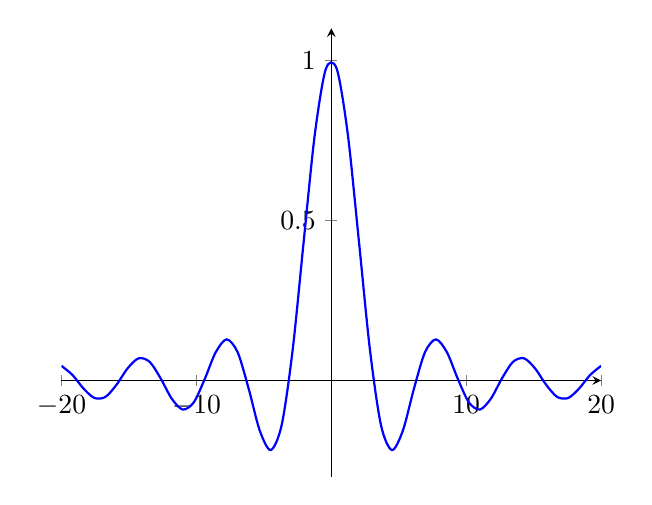
\begin{tikzpicture}
        \begin{axis}[
                axis lines=middle,
                %grid,
                %thick,
                domain=-20:20,
                xmin=-20,
                xmax=20,
                ymin=-0.3,
                ymax=1.1,
                %legend pos=outer north east,
                smooth,
            ]
            \addplot[
                domain=-20:20,
                samples=50,
                blue,
                thick]
            {sin(deg(x))/x};
        \end{axis}
    \end{tikzpicture}
\end{center}

\[Sa\p{t}=\frac{\sin t}t\]

\[\impint Sa\p{t}=\pi\]

\subsubsection{单位阶跃信号}

\[u\p{t}=
    \left\{\begin{aligned}
        0 &  & t<0 \\
        1 &  & t>0
    \end{aligned}\right.\]

\subsubsection{单位矩形脉冲信号}

\[g_T\p{t}=
    \left\{\begin{aligned}
        0 &  & \abs{t}>\frac T2 \\
        1 &  & \abs{t}<\frac T2
    \end{aligned}\right.\]

\[g_T\p{t}=u\p{t+\frac T2}-u\p{t-\frac T2}\]

\subsubsection{符号函数}

\[\mathrm{sgn}\p{t}=
    \left\{\begin{aligned}
        -1 &  & t<0 \\
        1  &  & t>0
    \end{aligned}\right.\]

\[\mathrm{sgn}\p{t}=2u\p{t}-1\]

\subsubsection{单位冲激信号(狄拉克函数)}

\[\delta\p{t}=
    \left\{\begin{aligned}
        +\infty &  & t=0    \\
        0       &  & t\neq0
    \end{aligned}\right.\]

\[\int_{0_-}^{0_+}\delta\p{t}\d t=1\]

\[\delta\p{t}=\frac{\d u\p{t}}{\d t}\]

\[\delta\p{at}=\frac1{\abs a}\delta\p{t}\p{a\neq0}\]

\[\delta\p{t-t_0}\ast\ft=f\p{t-t_0}\]

\subsection{离散信号}

\subsubsection{单位阶跃序列}

\[u\p{k}=
    \left\{\begin{aligned}
        0 &  & t<0         \\
        1 &  & t\geqslant0
    \end{aligned}\right.\]


\subsubsection{单位样值序列}

\[\delta\p{k}=
    \left\{\begin{aligned}
        1 &  & k=0    \\
        0 &  & k\neq0
    \end{aligned}\right.\]

\[\delta\p{k}=\nabla u\p{k}\]

\[\delta\p{k-k_0}\ast\fk=f\p{k-k_0}\]

\part{LTI时域分析}

\section{电路基础}

\subsection{电阻}

\[u_t=Ri_t\]

\subsection{电感}

\[u_t=Li_t^\prime\]

\[u_C\p{0_-}=u_C\p{0_+}\]

\subsection{电容}

\[i_t=Cu_t^\prime\]

\[i_L\p{0_-}=i_L\p{0_+}\]

\section{LTI电路}

本节中都有$k\in\{0,1,\cdots,n-1\}$

\subsection{符号定义}

\paragraph{激励(输入)信号}

$e\p{t}$或$\ft$

\paragraph{响应(输出)信号}

$r\p{t}$或$y\p{t}$

\paragraph{系统函数(系统冲激响应)}

$h\p{t}$

\paragraph{系统输入关系}

\[\ft\ast h\p{t}=y\p{t}\]

\paragraph{自由响应(固有响应)}

电路微分方程对应的齐次(通)解
$r_h\p{t}$

\paragraph{强迫响应}

电路微分方程对应的(非齐次)特解
$r_p\p{t}$

\paragraph{零输入响应}

$r_{zi}$或$y_x\p{t}$

\paragraph{零状态响应}

$r_{zs}$或$y_f\p{t}$

\paragraph{全响应}

电路微分方程对应的全解
$r\p{t}=r_h\p{t}+r_p\p{t}=r_{zi}\p{t}+r_{zs}\p{t}$

\subsection{起始状态}

\[r^{\p{k}}\p{0_-}\]

\subsection{初始状态}

\[r^{\p{k}}\p{0_+}\]

\subsection{零输入响应}

\[r_{zi}^{\p{k}}\p{0_+}
    =r_{zi}^{\p{k}}\p{0_-}
    =r^{\p{k}}\p{0_-}\]

\subsection{零状态响应}

\[r_{zs}^{\p{k}}\p{0_-}=0\]

\subsection{全响应分解}

\[\begin{aligned}
        r\p{t}
         & =\underbrace{\sum_{k=1}^nA_k\e^{\alpha_kt}}_\text{自由响应}
        +\underbrace{B\p{t}}_\text{强迫响应}                                 \\
         & =\underbrace{\sum_{k=1}^nA_{zik}\e^{\alpha_kt}}_\text{零输入响应}
        +\underbrace{\sum_{k=1}^nA_{zsk}\e^{\alpha_kt}+B\p{t}}_\text{零状态响应}
    \end{aligned}\]

\part{卷积}

\[\ft\ast g\p{t}
    =\impint
    f\p{\tau}g\p{t-\tau}\d\tau\]

\section{性质\label{连续卷积性质}}

\subsection{交换律}

\[f\ast g=g\ast f\]

\subsection{结合律}

\[\p{f\ast g}\ast h=f\ast\p{g\ast h}\]

\subsection{分配律}

\[f\ast\p{g+h}=f\ast g+f\ast h\]

\subsection{并联系统}

\[h=h_1+h_2\]

\subsection{串联(级联)系统}

\[h=h_1\ast h_2\]

\subsection{微积分性质}

\[s=f\ast g\implies s^{\p{i}}=f^{\p{j}}\ast g^{\p{i-j}}\]

\part{傅里叶变换}

\section{正交函数集}

\[\int_{t_1}^{t_2}\varphi_i\varphi_j\d t
    \left\{\begin{aligned}
        =0    &  & i\neq j \\
        \neq0 &  & i=j
    \end{aligned}\right.\]

\section{傅里叶级数}

\subsection{三角形式}

\[\begin{aligned}
        \ft
        = & \frac{a_0}2+\sum_{n\in\snp}\p{a_n\cos n\omega t+b_n\sin n\omega t} \\
        = & \frac{c_0}2+\sum_{n\in\snp}c_n\cos\p{n\omega t+\varphi_n}
    \end{aligned}\]

\paragraph{周期信号}$\ft$

\paragraph{周期}$T$

\paragraph{角频率}$\omega=\dfrac{2\pi}T$

\paragraph{频率}$f=T^{-1}$

\paragraph{直流分量(与书上不同)}$\dfrac{a_0}2=\dfrac{c_0}2\p{b_0=0}$

\paragraph{余弦分量的幅度}$\displaystyle a_n=\frac2T\int_{t_0}^{t_0+T}\ft\cos n\omega t\d t$

\paragraph{正弦分量的幅度}$\displaystyle b_n=\frac2T\int_{t_0}^{t_0+T}\ft\sin n\omega t\d t$

\paragraph{基波分量}$c_1\cos\p{n\omega t+\varphi_1}$

\paragraph{$n$次谐波分量}$c_n\cos\p{n\omega t+\varphi_n}$

\paragraph{其他关系}

\[\begin{aligned}
        a_n       & =c_n\cos\varphi_n        \\
        b_n       & =-c_n\sin\varphi_n       \\
        c_n       & =\sqrt{a_n^2+b_n^2}      \\
        \varphi_n & =-\arctan\frac{b_n}{a_n}
    \end{aligned}\]

\paragraph{奇函数性质}$\ft=-f\p{-t}\implies a_n=0$

\paragraph{偶函数性质}$\ft=f\p{-t}\implies b_n=0$

\paragraph{奇谐函数性质}

\[\ft=-f\p{t\pm\frac T2}
    \implies\left\{\begin{aligned}
        a_n & =
        \left\{\begin{aligned}
                    & 0                                             &  & n=2k   \\
                    & \frac4T\int_0^{\frac T2}\ft\cos n\omega t\d t &  & n=2k+1
               \end{aligned}\right. \\
        b_n & =
        \left\{\begin{aligned}
                    & 0                                             &  & n=2k   \\
                    & \frac4T\int_0^{\frac T2}\ft\sin n\omega t\d t &  & n=2k+1
               \end{aligned}\right.
    \end{aligned}\right.k\in\sz\]

\subsection{指数形式}

\[\ft=\sumsz F_n\e^{\j n\omega t}\]

\paragraph{复系数}$\displaystyle F_n=\frac1T\int_{t_0}^{t_0+T}\ft\e^{-\j n\omega t}\d t$

\paragraph{幅度谱}$\abs{F_n}\sim n\omega$

\paragraph{相位谱}$\varphi_n\sim n\omega$

\paragraph{其他关系}

\[F_{\pm n}=\abs{F_{\pm n}}\e^{\pm\j\varphi_n}=\frac12\p{a_n\mp\j b_n}\]

\[\abs{F_n}=\abs{F_{-n}}=\frac{c_n}2\]

\paragraph{功率}$\displaystyle P=\sumsz\abs{F_n}^2$

\subsection{周期矩形脉冲信号}

\paragraph{一个周期内}

\[\ft=
    \left\{\begin{aligned}
        E &  & \abs{t}            & \leqslant\frac\tau2 \\
        0 &  & \frac\tau2<\abs{t} & \leqslant\frac T2
    \end{aligned}\right.\]

\[a_n=c_n=\frac{2E\tau}TSa\p{\frac{n\omega\tau}2}\]

\[b_n=0\]

\[\begin{aligned}
        \ft & =\frac{E\tau}T+\frac{2E\tau}T\sum_{n\in\snp}Sa\p{\frac{n\omega\tau}2}\cos n\omega t \\
            & =\frac{E\tau}T\sumsz Sa\p{\frac{n\omega\tau}2}\e^{\j n\omega t}
    \end{aligned}\]

\section{傅里叶变换}

\paragraph{傅里叶变换}

\[\fw=\fourier\ft=\impint\ft\e^{-\j\omega t}\d t\]

\paragraph{傅里叶逆变换}

\[\ft=\ifourier{\fw}=\frac1{2\pi}\impint \fw\e^{\j\omega t}\d\omega\]

\paragraph{充分条件}

$\displaystyle\impint\abs\ft\d t<+\infty$

\paragraph{幅度谱}

$\abs{\fw}\sim\omega$

\paragraph{相位谱}

$\abs{\varphi\p{\omega}}\sim \omega$

\subsection{频带宽度}

\paragraph{$\tau$:等效脉冲宽度}

\[f\p{0}\tau=F\p{0}=\impint\ft\d t\]

\paragraph{$B$:等效频带宽度}

\[F\p{0}B_\omega=2\pi f\p{0}=\impint \fw\d\omega\]

\[B_\omega=\frac{2\pi}\tau\]

\[B_f=\frac1\tau\]

\subsection{典型非周期信号傅里叶变换}

\subsubsection{单边指数信号}

\[\ft=\e^{-\alpha t}u\p{t}\]

\[\left\{\begin{aligned}
        \fw               & =\frac1{\alpha+\j\omega}          \\
        \abs{\fw}         & =\frac1{\sqrt{\alpha^2+\omega^2}} \\
        \varphi\p{\omega} & =-\arctan\frac\omega\alpha
    \end{aligned}\right.\]

\subsubsection{双边指数信号}

\[\ft=\e^{-\alpha\abs t}\]

\[\left\{\begin{aligned}
        \fw               & =\frac{2\alpha}{\alpha^2+\omega^2} \\
        \abs{\fw}         & =\frac{2\alpha}{\alpha^2+\omega^2} \\
        \varphi\p{\omega} & =0
    \end{aligned}\right.\]

\subsubsection{矩形脉冲信号}

\[\ft=E\cdot g_T\p{t}\]

\[\fw=E\tau\cdot Sa\p{\frac{\omega\tau}2}\]

\[B_f=\frac1\tau\]

\subsubsection{符号函数}

\[\ft=\mathrm{sgn}\p{t}\]

\[\left\{\begin{aligned}
        \fw               & =\frac2{\j\omega}   \\
        \abs{\fw}         & =\frac2{\abs\omega} \\
        \varphi\p{\omega} & =
        \left\{\begin{aligned}
                   \frac\pi2  &  & \omega<0 \\
                   -\frac\pi2 &  & \omega>0
               \end{aligned}\right.
    \end{aligned}\right.\]

\subsection{常用变换对}

\[\begin{tblr}{c|c}
        \hline
        \ft                  & \fw                                                          \\
        \hline
        1                    & 2\pi\delta\p{\omega }                                        \\
        \delta\p{t}          & 1                                                            \\
        u\p{t}               & \pi\delta\p{\omega}+\dfrac1{\j\omega}                        \\
        \e^{-\alpha t}u\p{t} & \dfrac1{\alpha+\j\omega}                                     \\
        \e^{-\alpha\abs t}   & \dfrac{2\alpha}{\alpha^2+\omega^2}                           \\
        g_\tau\p{t}          & \tau\cdot Sa\p{\dfrac{\omega\tau}2}                          \\
        \mathrm{sgn}\p{t}    & \dfrac2{\j\omega}                                            \\
        \e^{\j\omega_0t}     & 2\pi\delta\p{\omega-\omega_0}                                \\
        \cos\omega_0 t       & \pi\p{\delta\p{\omega+\omega_0}+\delta\p{\omega-\omega_0}}   \\
        \sin\omega_0 t       & \j\pi\p{\delta\p{\omega+\omega_0}-\delta\p{\omega-\omega_0}} \\
        \hline
    \end{tblr}\]

\subsection{性质}

\[\fourier{\ft}=\fw\]

\subsubsection{线性}

\[\fourier{f+g}=\fourier f+\fourier g\]

\subsubsection{对称性}

\[\fourier{\fourier\ft}=2\pi f\p{-\omega}\]

\subsubsection{奇偶虚实性}

略

\subsubsection{尺度变换特性}

\[\fourier{f\p{at}}=\frac1{\abs a}F\p{\frac\omega a}\]

\subsubsection{时移特性}

\[\fourier{f\p{t+t_0}}=\e^{\j\omega t_0}\cdot \fw\]

\subsubsection{频移特性}

\[\fourier{\ft\e^{-\j\omega_0t}}=F\p{\omega+\omega_0}\]

\paragraph{频谱搬移}

\[\fourier{\ft\cos\omega_0t}
    =\fourier{\frac\ft2\p{\e^{\j\omega t}+\e^{-\j\omega t}}}
    =\frac12\p{F\p{\omega+\omega_0}+F\p{\omega-\omega_0}}\]

下式不常用

\[\fourier{\ft\sin\omega_0t}
    =\fourier{\frac\ft{2\j}\p{\e^{\j\omega t}-\e^{-\j\omega t}}}
    =\frac\j2\p{F\p{\omega+\omega_0}-F\p{\omega-\omega_0}}\]

\subsubsection{时域微分特性}

\[\fourier{f^{\p{n}}\p{t}}=\p{\j\omega}^n\cdot \fw\]

\subsubsection{频域微分特性}

\[\fourier{\p{\j t}^n\cdot\ft}=F^{\p{n}}\p{\omega}\]

\subsubsection{时域积分特性}

\[\fourier{\int\limits_{-\infty}^tf\p{\tau}\d\tau}=\frac{\fw}{\j\omega}+\pi F\p{0}\delta\p{\omega}\]

\subsubsection{频域积分特性}

略

\subsubsection{时域卷积特性}

\[\fourier{f\ast g}=\fourier f\cdot\fourier g\]

\subsubsection{频域卷积特性}

\[\fourier{f\cdot g}=\frac1{2\pi}\fourier f\ast\fourier g\]

\subsection{周期信号傅里叶变换}

$\ft$角频率为$\omega_0$,第一个周期的频域$F_0\p{\omega}$

\[\fw=2\pi\sumsz F_n\delta\p{\omega-n\omega_0}\]

\[F_n=\left.\frac1TF_0\p{\omega}\right|_{\omega=n\omega_0}=\left.\frac1T\int_{-\frac T2}^{\frac T2}\ft\e^{-\j\omega t}\d t\right|_{\omega=n\omega_0}\]

\subsection{抽样信号的傅里叶变换}

抽样信号$=$连续信号$\cdot$抽样脉冲

\[f_s\p{t}=\ft p\p{t}\]

\[P\p{\omega}=2\pi\sumsz P_n\delta\p{\omega-n\omega_s}\]

\[F_s\p{\omega}=\frac1{2\pi}\fw\ast P\p{\omega}=\sumsz P_nF\p{\omega-n\omega_s}\]

\subsubsection{均匀抽样脉冲}

$p\p{t}$角频率(抽样频率)为$\omega_s$,周期(抽样周期)为$T_s$

\paragraph{冲激抽样}

\[\delta_T\p{t}=\sumsz\delta\p{t-nT_s}\]

\[\left\{\begin{aligned}
        P_n           & =\frac1T_s                                \\
        \delta_T\p{t} & =\frac1{T_s}\sumsz\e^{\j n\omega_s t}     \\
        P\p{\omega}   & =\omega_s\sumsz\delta\p{\omega-n\omega_s}
    \end{aligned}\right.\]

\[F_s\p{\omega}=\frac1{T_s}\sumsz F\p{\omega-n\omega_s}\]

\paragraph{矩形脉冲(自然)抽样}

\[\delta_T\p{t}=\sumsz\delta\p{t-nT_s}\]

\[P_n=\frac{E\tau}{T_s}Sa\p{\frac{n\omega_s\tau}2}\]

\[F_s\p{\omega}=\frac{E\tau}{T_s}\sumsz Sa\p{\frac{n\omega_s\tau}2}F\p{\omega-n\omega_s}\]

\subsubsection{时域抽样定理}

\paragraph{奈奎斯特频率}

\[f_s\geqslant2f_m\]

\paragraph{奈奎斯特周期}

\[T_s\leqslant\frac1{2f_m}\]

\subsubsection{LTI系统的频域分析}

\[Y_f\p{\omega}=\fourier{y_f\p{t}}=\fw H\p{\omega}\]

\part{拉普拉斯变换}

$s=\sigma+\j\omega$

\section{拉普拉斯变换}

\paragraph{双边拉普拉斯变换}

\[\fs=\laplace{\ft}=\impint\ft\e^{-st}\d t\]

\paragraph{单边拉普拉斯变换(以下拉普拉斯变换都指单边)}

\[\fs=\laplace{\ft}=\int\limits_0^{+\infty}\ft\e^{-st}\d t\]

\paragraph{拉普拉斯逆变换}

\[\ft=\ilaplace{\fs}=\frac1{2\pi\j}\int_{\sigma-\j\infty}^{\sigma+\j\infty}\fs\e^{st}\d s\]

\subsection{常用变换对}

定义域$D\subseteq\srp$,收敛域$\sigma>\sigma_0$

\[\begin{tblr}{c|c|c}
        \hline
        \ft                         & \fs                                         & \sigma_0 \\
        \hline
        t^n                         & \dfrac{n!}{s^{n+1}}                         & 0        \\
        \e^{-\lambda t}             & \dfrac1{s+\lambda}                          & -\lambda \\
        \e^{\j\omega t}             & \dfrac1{s-\j\omega}                         & 0        \\
        \cos\omega t                & \dfrac s{s^2+\omega^2}                      & 0        \\
        \sin\omega t                & \dfrac\omega{s^2+\omega^2}                  & 0        \\
        \delta^{\p{n}}\p{t}         & s^n                                         & -\infty  \\
        t^n\e^{-\lambda t}          & \dfrac{n!}{\p{s+\lambda}^{n+1}}             & -\lambda \\
        \e^{-\lambda t}\cos\omega t & \dfrac{s+\lambda}{\p{s+\lambda}^2+\omega^2} & -\lambda \\
        \e^{-\lambda t}\sin\omega t & \dfrac\omega{\p{s+\lambda}^2+\omega^2}      & -\lambda \\
        t\cos\omega t               & \dfrac{s^2-\omega^2}{\p{s^2+\omega^2}^2}    & 0        \\
        t\sin\omega t               & \dfrac{2\omega s}{\p{s^2+\omega^2}^2}       & 0        \\
        \hline
    \end{tblr}\]

\subsection{性质}

以下函数收敛域

\[\begin{aligned}
        \laplace{f} & :\sigma>\sigma_1 \\
        \laplace{g} & :\sigma>\sigma_2
    \end{aligned}\]

\[\laplace{\ft}=\fs\]

\subsubsection{线性}

\[\laplace{f+g}=\laplace{f}+\laplace{g}
    \p{\sigma>\max\p{\sigma_1,\sigma_2}}\]

\subsubsection{尺度变换特性}

\[\laplace{f\p{at}}=\frac1aF\p{\frac sa}
    \p{\sigma>a\sigma_1}\]

\subsubsection{时移特性}

\[\laplace{f\p{t-t_0}}=\e^{-st_0}\fs\p{t_0\geqslant0}
    \p{\sigma>\sigma_1}\]

\subsubsection{复频域平移特性}

\[\laplace{\e^{-\lambda t}\ft}=F\p{s+\lambda}
    \p{\sigma>\sigma_1-\lambda}\]

\subsubsection{时域微分特性}

\[\laplace{f^{\p{n}}\p{t}}=s^n\fs-\sum_{r=0}^{n-1}s^{n-r-1}f^r\p{0}
    \p{\sigma>\sigma_1}\]

\subsubsection{复频域微分特性}

\[\laplace{\p{-t}^n\ft}=F^{\p{n}}\p{s}
    \p{\sigma>\sigma_1}\]

\subsubsection{时域积分特性}

\[\laplace{\int\limits_{-\infty}^tf\p{\tau}\d\tau}=
    \frac1s\p{\fs+\int\limits_{-\infty}^0f\p{\tau}\d\tau}
    \p{\sigma>\max\p{\sigma_1,0}}\]

\subsubsection{复频域积分特性}

略

\subsubsection{时域卷积特性}

\[\laplace{f\ast g}=\laplace{f}\cdot\laplace{g}
    \p{\sigma>\max\p{\sigma_1,\sigma_2}}\]

\subsubsection{复频域卷积特性}

\[\laplace{f\cdot g}=
    \frac1{2\pi\j}\laplace{f}\ast\laplace{g}
    \p{\sigma>\sigma_1+\sigma_2}\]

\subsubsection{初值定理}

\[\lim_{t\to0^+}\ft=f\p{0^+}=\lim_{s\to+\infty}s\fs\]

\subsubsection{终值定理}

\[\lim_{t\to+\infty}\ft=f\p{+\infty}=\lim_{s\to0}s\fs\]

\section{拉普拉斯逆变换}

\subsection{部分分式展开法\label{拉普拉斯变换部分分式展开法}}

\paragraph{有理分式}

\[\fs=\frac{\mathcal P_m\p{s}}{\mathcal Q_n\p{s}}
    =\frac{\sum\limits_{i=0}^mb_is^i}{\sum\limits_{i=0}^na_is^i}\]

\paragraph{若为有理真分式($m<n$)}

\[\fs=\frac{\mathcal P_m\p{s}}{\prod\limits_{i=1}^n\p{s-p_i}}\]

\subparagraph{若$s=p_i$项都为一阶极点}

可分解为:

\[\fs=\sum_{i=1}^n\frac{k_i}{s-p_i}\]

\[k_i=\left.\p{s-p_i}\fs\right|_{s=p_i}\p{1\leqslant i\leqslant n}\]

\subparagraph{若$s=u$项为$r$重阶极点}

可分解为:

\[\fs=\frac{\mathcal P_m\p{s}}{{\p{s-u}}^r\cdot\prod\limits_{i=1}^{n-r}\p{s-p_i}}
    =\sum_{j=1}^r\frac{q_j}{{\p{s-u}}^j}+\sum_{i=1}^{n-r}\frac{k_i}{s-p_i}\]

\[\left\{\begin{aligned}
        q_j & =\left.\frac1{\p{r-j}!}{\p{\frac\d{\d s}}}^{r-j}\left[{\p{s-u}}^r\fs\right]\right|_{s=u} &  & 1\leqslant j\leqslant r   \\
        k_i & =\left.\p{s-p_i}\fs\right|_{s=p_i}                                                       &  & 1\leqslant i\leqslant n-r
    \end{aligned}\right.\]

\paragraph{若为有理假分式($m\geqslant n$)}

\[\fs=\sum_{i=0}^{m-n}B_is^i+\frac{\mathcal R_{n-1}\p{s}}{\mathcal Q_n\p{s}}\]

后按有理真分式变换

\subsection{留数法}

略

\section{连续系统响应的复频域分析}

\subsection{二阶LTI系统响应}

\paragraph{激励方程}

\[a_0y\p{t}+a_1y^\prime\p{t}+a_2y^{\prime\prime}\p{t}
    =b_0\ft+b_1f^\prime\p{t}+b_2f^{\prime\prime}\p{t}\]

\[\sum_{i=0}^na_iy^{\p{i}}\p{t}
    =\sum_{i=0}^nb_if^{\p{i}}\p{t}\]

\paragraph{拉普拉斯变换后}

\[\underbrace{a_0Y\p{s}}_{\laplace{a_0y\p{t}}}
    +\underbrace{a_1\left[{sY\p{s}-y\p{0_-}}\right]}_{\laplace{a_1y^\prime\p{t}}}
    +\underbrace{a_2\left[{s^2Y\p{s}-sy\p{0_-}-y^\prime\p{0_-}}\right]}_{\laplace{a_2y^{\prime\prime}\p{t}}}
    =\underbrace{b_0\fs}_{\laplace{b_0\ft}}
    +\underbrace{b_1s\fs}_{\laplace{b_1f^\prime\p{t}}}
    +\underbrace{b_2s^2\fs}_{\laplace{b_2f^{\prime\prime}\p{t}}}\]

\[\sum_{i=0}^na_i\p{s^iY\p{s}+\sum_{j=0}^{i-1}s^{i-1-j}y^{\p{j}}\p{0_-}}
    =\sum_{i=0}^nb_is^i\fs\]

\paragraph{全响应}

\[Y\p{s}
    =\underbrace{\frac{a_2\left[sy\p{0_-}+y^\prime\p{0_-}\right]+a_1y\p{0_-}}{a_2s^2+a_1s+a_0}}_{Y_x\p{s}}
    +\underbrace{\overbrace{\frac{b_2s^2+b_1s+b_0}{a_2s^2+a_1s+a_0}}^{H\p{s}}\fs}_{Y_f\p{s}}\]

\subparagraph{零输入响应}

$y_x\p{t}=\ilaplace{Y_x\p{s}}$

\subparagraph{零状态响应}

$y_f\p{t}=\ilaplace{Y_f\p{s}}$

\subsection{电路的复频域模型}

\[\begin{tblr}{c|c|c}
        \hline
        \text{元件} & \text{时域}     & \text{复频域}            \\
        \hline
        \text{电阻} & u_t=Ri_t        & U_s=RI_s                 \\
        \text{电感} & u_t=Li_t^\prime & U_s=L\p{sI_s-i_t\p{0_-}} \\
        \text{电容} & i_t=Cu_t^\prime & I_s=C\p{sU_s-u_t\p{0_-}} \\
        \hline
    \end{tblr}\]

\subsection{串联形式的复频域模型}

$U_s$为两端电势差

\paragraph{电阻}

\[\begin{circuitikz}[european resistors]
        \draw(-2,0)
        to[R=$R$,i=$I_s$,o-o](2,0);
    \end{circuitikz}\]

\paragraph{电感}

\[\begin{circuitikz}
        \draw(-2,0)
        to[L=$sL$,i=$I_s$,o-](0,0)
        to[V=$Li_t\p{0_-}$,-o](2,0);
    \end{circuitikz}\]

\paragraph{电容}

\[\begin{circuitikz}
        \draw(-2,0)
        to[C=${\p{sC}}^{-1}$,i=$I_s$,o-](0,0)
        (2,0)
        to[V=$s^{-1}u_t\p{0_-}$,o-](0,0);
    \end{circuitikz}\]

\subsection{LTI系统的复频域分析}

\[Y_f\p{s}=\fourier{y_f\p{t}}=\fs H\p{s}\]

\section{零极点}

类似于\ref{拉普拉斯变换部分分式展开法}

\[H\p{s}=\frac{\mathcal P_m\p{s}}{\mathcal Q_n\p{s}}
    =K\frac{\prod\limits_{i=1}^m\p{s-z_i}}
    {\prod\limits_{i=1}^n\p{s-p_i}}\]

\paragraph{零点}$z_i$

\paragraph{极点}$p_i$

\subsection{系统稳定性}

稳定系统充要条件(绝对可积条件)

\[\impint\abs{h\p{t}}\d t<+\infty\]

\subsubsection{不稳定系统}

存在极点的实部大于等于0

\[\exists p_i,\sigma_{p_i}\geqslant0\]

或

存在多阶极点的实部等于0

\[\exists p_i=p_j\to\sigma_{p_i}=0\]

\subsubsection{临界稳定系统}

所有极点实部都小于等于0

\[\forall p_i=p_j\to\sigma_{p_i}\leqslant0\]

并且

极点的实部等于0的都是一阶极点

\[\forall\sigma_{p_i}=\sigma_{p_j}=0;p_i=p_j\to i=j\]

\subsubsection{稳定系统}

所有极点实部都小于0

\[\forall p_i,\sigma_{p_i}<0\]

\section{频响特性}

系统稳定时,令$s=\j\omega$(即退化为傅里叶变换后的频域响应)

\[H\p{\omega}=\abs{H\p{\omega}}\varphi\p{\omega}\]

\paragraph{幅频特性}$\abs{H\p{\omega}}$

\paragraph{相频特性}$\varphi\p{\omega}$

\part{离散系统时域分析}

\section{LTI离散系统的响应}

\subsection{差分}

\paragraph{一阶前向差分}

\[\Delta\fk=f\p{k+1}-\fk\]

\paragraph{一阶后向差分(以下差分都指后向差分)}

\[\nabla\fk=\fk-f\p{k-1}\]

\subsection{性质}

\subsubsection{线性}

\[\nabla\p{f+g}=\nabla f+\nabla g\]

\subsubsection{多阶差分}

\[\begin{aligned}
        \nabla^2\fk & =\nabla\p{\nabla\fk}=\fk-2f\p{k-1}+f\p{k-2} \\
        \nabla^n\fk & =\fk+\sum_{i=1}^nb_if\p{k-i}
    \end{aligned}\]

\subsection{零输入响应}

\[y_x\p{k}=y\p{k}\p{k<0}\]

\subsection{零状态响应}

\[y_f\p{k}=0\p{k<0}\]

\section{卷积和}

\[f\p{k}\ast g\p{k}=\sumsz f\p{n}g\p{k-n}\]

\subsection{性质}

除了微积分性质变为差分性质,其他与连续性质(\ref{连续卷积性质})相同

\subsubsection{差分性质}

\[\begin{aligned}
        s\p{n}=f\p{k}\ast g\p{k} & \implies\nabla^is\p{k}=\nabla^jf\p{k}\ast\nabla^{i-j}g\p{k} \\
                                 & \implies E^{-i}s\p{k}=E^{-j}f\p{k}\ast E^{-\p{i-j}}g\p{k}
    \end{aligned}\]

\section{位移算子分析}

\[E^n\fk=f\p{k+n}\p{n\in\sz}\]

\part{Z变换}

$z=\e^{sT}$

\section{Z变换}

\paragraph{双边Z变换}

\[\fz=\ztrans{\fk}=\sum_{k\in\sz}\fk z^{-k}\]

\paragraph{单边Z变换(以下Z变换都指单边)}

\[\fz=\ztrans{\fk}=\sum_{k\in\sn}\fk z^{-k}\]

\paragraph{Z逆变换}

\[\fk=\iztrans{\fz}=\frac1{2\pi\j}\oint_C\fz z^{k-1}\d z\]

\subsection{常用变换对}

定义域$D\in\sn$,收敛域$\abs{z}>\abs{R_f}$

$-$表示$\abs{z}\geqslant0$

\[\begin{tblr}{c|c|c}
        \hline
        \fk             & \fz                                           & R_f \\
        \hline
        \delta\p{k}     & 1                                             & -   \\
        1               & \dfrac1{1-z^{-1}}                             & 1   \\
        k               & \dfrac z{{\p{z-1}}^2}                         & 1   \\
        \e^{\j\omega k} & \dfrac1{1-\e^{\j\omega}z^{-1}}                & 1   \\
        \cos\omega k    & \dfrac{z\p{z-\cos\omega}}{z^2-2z\cos\omega+1} & 1   \\
        \sin\omega k    & \dfrac{z\sin\omega}{z^2-2z\cos\omega+1}       & 1   \\
        a^k             & \dfrac1{1-az^{-1}}                            & a   \\
        ka^k            & \dfrac{az}{{\p{z-a}}^2}                       & a   \\
        \hline
    \end{tblr}\]

\subsection{性质}

以下函数收敛域

\[\begin{aligned}
        \ztrans{f} & :\abs{z}>R_{f1} \\
        \ztrans{g} & :\abs{z}>R_{f2}
    \end{aligned}\]

\[\ztrans{\fk}=\fz\]

\subsubsection{线性}

\[\ztrans{f+g}=\ztrans{f}+\ztrans{g}\p{\abs{z}>\max\p{{R_{f1},R_{f2}}}}\]

\subsubsection{指数加权(尺度变换)特性}

\[\ztrans{a^k\fk}=F\p{\frac za}\p{\abs z>\abs aR_{f1}}\]

\subsubsection{序列平移特性}

\[\ztrans{f\p{k+k_0}}=z^{k_0}\fz\p{\abs{z}>R_{f1}}\]

\subsubsection{Z域微分特性}

\[\ztrans{k\fk}=-zF^\prime\p{z}\p{\abs{z}>R_{f1}}\]

\subsubsection{序列卷积特性}

\[\ztrans{f\ast g}=\ztrans{g}\cdot\ztrans{g}\p{\abs{z}>\max\p{{R_{f1},R_{f2}}}}\]

\subsubsection{初值定理}

\[f\p{0}=\lim_{z\to\infty}\fz\]

\subsubsection{终值定理}

\[f\p{\infty}=\lim_{z\to1}\p{z-1}\fz\]

\section{Z逆变换}

\subsection{部分分式展开法\label{Z变换部分分式展开法}}

\paragraph{有理分式}

\[\fz=\frac{\mathcal P_m\p{z^{-1}}}{\mathcal Q_n\p{z^{-1}}}
    =\frac{\sum\limits_{i=0}^mb_iz^{-i}}{\sum\limits_{i=0}^na_iz^{-i}}\]

\paragraph{若为有理真分式($m<n$)}

\[\fz=\frac{\mathcal P_m\p{z^{-1}}}{\prod\limits_{i=1}^n\p{1-p_iz^{-1}}}\]

\subparagraph{若$z=p_i$项都为一阶极点}

可分解为:

\[\fz=\sum_{i=1}^n\frac{k_i}{1-p_iz^{-1}}\]

\[k_i=\left.\p{1-p_iz^{-1}}\fz\right|_{z=p_i}\p{1\leqslant i\leqslant n}\]

\subparagraph{若$z=u$项为$r$重阶极点}

可分解为:

\[\fz=\frac{\mathcal P_m\p{z^{-1}}}{{\p{1-uz^{-1}}}^r\cdot\prod\limits_{i=1}^{n-r}\p{1-p_iz^{-1}}}
    =\sum_{j=1}^r\frac{q_j}{{\p{1-p_1z^{-1}}}^j}+\sum_{i=1}^{n-r}\frac{k_i}{1-p_iz^{-1}}\]

\[\left\{\begin{aligned}
        q_j & =\left.\frac1{{\p{-u}^{r-j}}\p{r-j}!}{\p{\frac\d{\d\p{z^{-1}}}}}^{r-j}\left[{\p{1-uz^{-1}}}^r\fz\right]\right|_{z=u} &  & 1\leqslant j\leqslant r   \\
        k_i & =\left.\p{1-p_iz^{-1}}\fz\right|_{z=p_i}                                                                             &  & 1\leqslant i\leqslant n-r
    \end{aligned}\right.\]

\paragraph{若为有理假分式($m\geqslant n$)}

\[\fs=\sum_{i=0}^{m-n}B_iz^{-i}+\frac{\mathcal R_{n-1}\p{z^{-1}}}{\mathcal Q_n\p{z^{-1}}}\]

后按有理真分式变换

\subsection{留数法}

略

\subsection{长除法}

略

\section{离散系统响应的Z域分析}

\subsection{二阶LTI系统响应}

\paragraph{激励方程}

\[a_0y\p{k}+a_1E^{-1}y\p{k}+a_2E^{-2}y\p{k}
    =b_0\fk+b_1E^{-1}\fk+b_2E^{-2}\fk\]

\paragraph{Z变换后}

\[\underbrace{a_0Y\p{z}}_{\ztrans{a_0y\p{k}}}
    +\underbrace{a_1\left[{z^{-1}Y\p{z}+y\p{-1}}\right]}_{\ztrans{a_1E^{-1}y\p{k}}}
    +\underbrace{a_2\left[{z^{-2}Y\p{z}+z^{-1}y\p{-1}+y\p{-2}}\right]}_{\ztrans{a_2E^{-2}y\p{k}}}\]

\[=\underbrace{b_0\fz}_{\ztrans{b_0\fk}}
    +\underbrace{b_1z^{-1}\fz}_{\ztrans{b_1E^{-1}\fk}}
    +\underbrace{b_2z^{-2}\fz}_{\ztrans{b_2E^{-2}\fk}}\]

\paragraph{全响应}

\[Y\p{z}
    =\underbrace{-\frac{a_2\left[z^{-1}y\p{-1}+y\p{-2}\right]+a_1y\p{-1}}{a_2z^{-2}+a_1z^{-1}+a_0}}_{Y_x\p{z}}
    +\underbrace{\overbrace{\frac{b_2z^{-2}+b_1z^{-1}+b_0}{a_2z^{-2}+a_1z^{-1}+a_0}}^{H\p{z}}\fz}_{Y_f\p{z}}\]

\subparagraph{零输入响应}

$y_x\p{t}=\iztrans{Y_x\p{z}}$

\subparagraph{零状态响应}

$y_f\p{t}=\iztrans{Y_f\p{z}}$

\section{零极点}

类似于\ref{Z变换部分分式展开法}

\[H\p{z}=\frac{\mathcal P_m\p{z}}{\mathcal Q_n\p{z}}
    =K\frac{\prod\limits_{i=1}^m\p{z-z_i}}
    {\prod\limits_{i=1}^n\p{z-p_i}}\]

\paragraph{零点}$z_i$

\paragraph{极点}$p_i$

\[R_f>\max\left\{z_i\right\}\]

\subsection{系统稳定性}

稳定系统充要条件(绝对可积条件)

\[\sum_{k\in\sz}\abs{h\p{k}}<+\infty\]

\subsubsection{不稳定系统}

有极点均在单位圆外

\[\exists p_i\to\abs{p_i}>1\]

或

存在多阶段极点在单位圆上

\[\exists p_i=p_j\to\abs{p_i}=1\]

\subsubsection{临界稳定系统}

所有极点都位于单位圆内

\[\forall p_i\to\abs{p_i}\leqslant1\]

并且

位于单位圆上的极点都是一阶极点

\[\forall\abs{p_i}=\abs{p_j}=1;p_i=p_j\to i=j\]

\subsubsection{稳定系统}

$H\p{z}$的收敛域包含单位圆(即所有极点均在单位圆内)

\[R_f>1\]

或(等价于)

\[\forall p_i\to\abs{p_i}<1\]

\end{document}
